\chapter{Aplicaciones existentes}
\label{cap:aplicacionesexistentes}

En este apartado se describen aplicaciones existentes y actuales que permiten que el proceso de calificación del alumnado sea más sencillo e intuitivo. En este capítulo se exponen algunas de ellas, y al final, se comparan con la que se ha desarrollado en este documento.

\section{EducamosCLM}

Esta aplicación web de la Junta de Comunidades de Castilla-La Mancha\cite{educamosclm} es la aplicación de gestión de alumnado por excelencia en los colegios públicos. 

Busca dotar de herramientas de gestión y comunicación para el profesorado, el alumnado y los padres mediante un entorno seguro, flexible e intuitivo. Además también posee un módulo para realizar trámites en las escuelas.

\begin{figure}[h]
\centering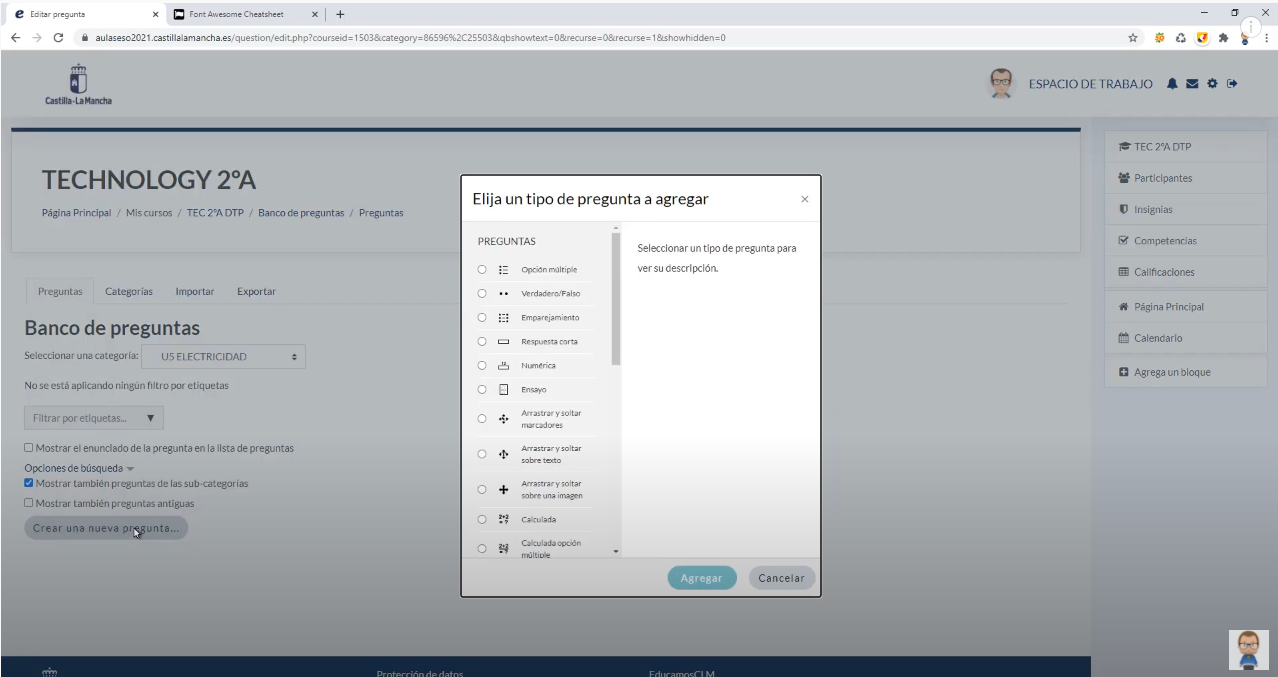
\includegraphics[width=1\linewidth]{figs/educamosCLM2.png}
\caption{Crear un examen en EducamosCLM.\cite{educamosclmyoutube}}
\label{Fig:educamosCLM}
\end{figure}

A continuación se muestran las características principales de EducamosCLM comparadas con las de esta aplicación. Cabe mencionar que, la primera y la que se ha considerado más notoria, es que EducamosCLM es exclusiva para los colegios públicos de Castilla-La Mancha, mientras que la desarrollada es libre y se podría usar en cualquier colegio sin restricciones regionales, público o privado.

\textbf {Seguimiento del curso.}
    En este apartado, los maestros pueden publicar las notas de sus alumnos para que estos y los padres las vean en cualquier momento, así como las faltas de asistencia y la trayectoria escolar que lleva el alumno durante el curso.
    En la vista de los alumnos, estos podrán subir sus trabajos on-line, que le aparecerán al maestro para que pueda descargarlos e introducir la calificación en el sistema. Este sistema también permite a los alumnos pedir tutorías con los maestros.
    
Usando la aplicación desarrollada, los maestros también podrán calificar a sus alumnos. El hecho de la comunicación externa con padres y alumnos es un módulo que está fuera del dominio y de los requisitos de esta aplicación.

\textbf {Personalización.} Otra diferencia notoria es la personalización. Mientras que EducamosCLM tiene una interfaz rígida y monótona, la aplicación desarrollada tiene varias opciones de personalización que se adaptan a cada maestro, entre las que se incluyen un tema oscuro y una selección especial de colores para personas daltónicas.


\section{Google Classroom}

Google Classroom es una aplicación para navegador web y para smartphone\cite{googleclassroom} desarrollada por Google que permite la comunicación entre maestros y alumnos, así como la gestión y organización de trabajos mediante Google Drive.

\begin{figure}[h]
\centering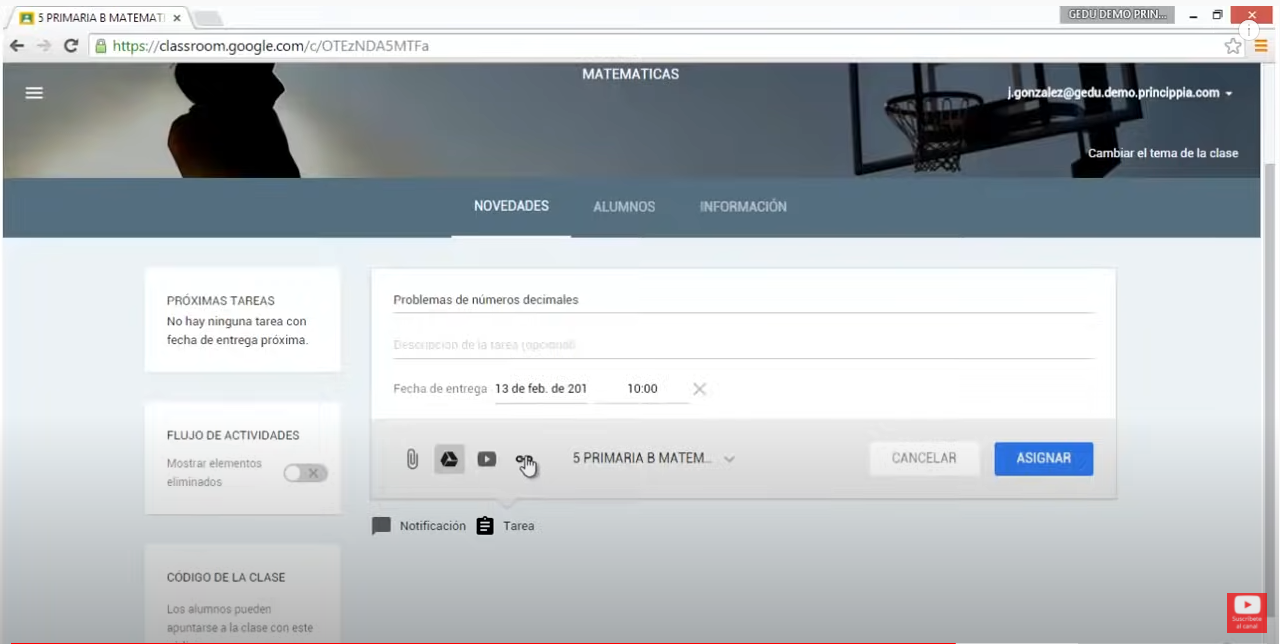
\includegraphics[width=1\linewidth]{figs/googleclassroom.png}
\caption{Crear una tarea en Google Classroom.\cite{googleclassroomyoutube}}
\label{Fig:googleclassroom}
\end{figure}

A continuación se muestran las características principales de Google Classroom comparadas con las de esta aplicación.

\textbf {Orientado a maestros y alumnos.} Principalmente, Google Classroom está pensado tanto para maestros como para alumnos, por lo que es muy completo. Tiene herramientas para programar entregas, reuniones y para que el maestro pueda comunicarse mediante mensajes de texto con un alumno o con toda la clase. En el alcance de la aplicación desarrollada no está la comunicación entre maestro y alumnos por las razones mencionadas en la sección anterior. Además, su propósito principal no es la organización de las clases, sino de los documentos de los docentes.

\textbf {Archivos en la nube.} Todos los archivos que se suben van directamente a Google Drive. De esta forma se almacenan todos en el mismo sitio, pero de forma ordenada, y cada alumno y docente puede acceder a estos archivos mediante una cuenta Google aceptada en el curso. La aplicación desarrollada no ha tenido en cuenta los trabajos on-line porque no se conecta a Internet, lo que permite que los datos a los que se acceden desde que el maestro inicia sesión, sean totalmente seguros y solo visibles por el propio docente.

\textbf {Personalizable mediante aplicaciones externas.} Google Classroom es una aplicación flexible: permite la integración de aplicaciones como Classcraft, Pear Deck o Quizizz, posibilitando una completa personalización de la experiencia tanto para los alumnos como para los maestros. Debido a la generalización de la herramienta, es muy versátil y se puede usar para cualquier curso, tanto de primaria como de secundaria. La aplicación desarrollada no contiene módulos descargables pero, una vez más, se puede hacer mención a la personalización de su interfaz, algo que Google Classroom tampoco tiene.
	

\section{Additio}
\label{sec:additio}

Additio es una aplicación para navegador web y smartphone\cite{additio} que permite gestionar las notas del alumnado y las competencias que tiene cada metodología, planificar las clases y la comunicación con padres y alumnos.

\begin{figure}[h]
\centering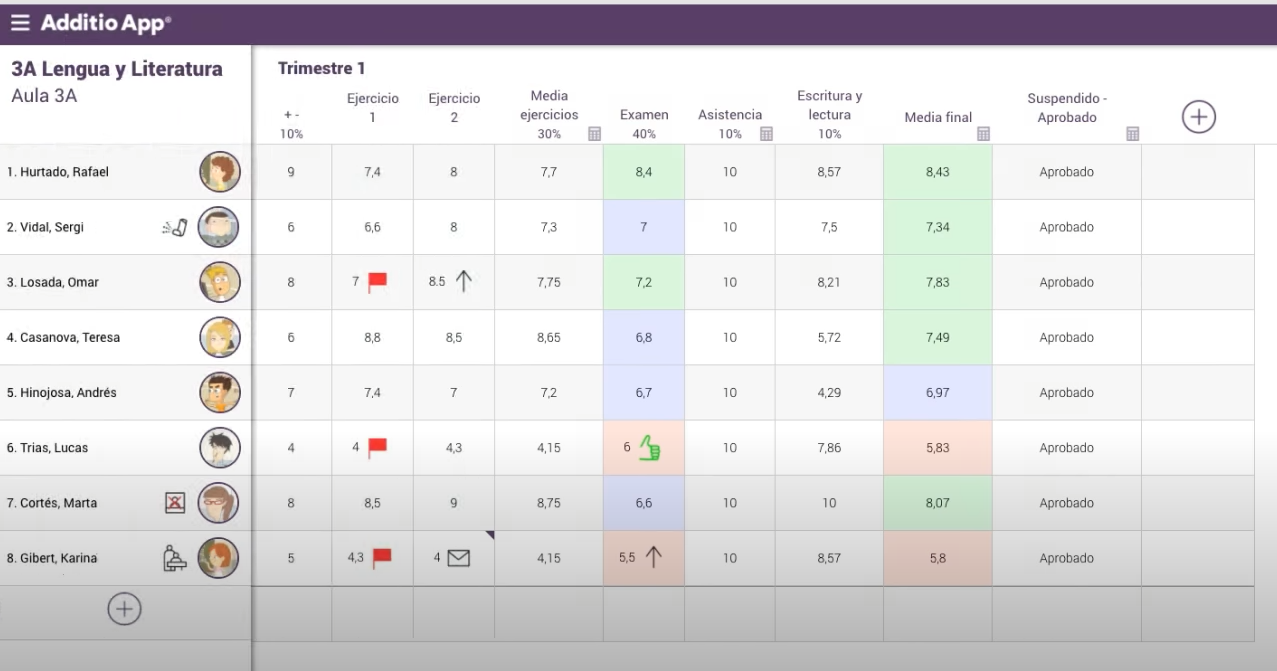
\includegraphics[width=1\linewidth]{figs/additio.png}
\caption{Gestión de notas en Additio.\cite{additioyoutube}}
\label{Fig:additio}
\end{figure}

A continuación se muestran las características principales de Additio comparadas con las de la aplicación desarrollada en este documento.

Additio es, de las aplicaciones que se han mostrado hasta ahora, la que más parecido tiene con la desarrollada en este documento. Está diseñada tanto para maestros como para Centros y permite, como las anteriores, gestionar notas y trabajos, la asistencia a clase y la comunicación entre padres, maestros y alumnos. Sin embargo, tiene una característica nueva que no se había encontrado en las aplicaciones descritas anteriormente: la posible introducción de competencias para las pruebas, funcionalidad que la aplicación desarrollada también posee.

\textbf {Varias funcionalidades.} La principal diferencia entre las dos aplicaciones es que la desarrollada, al contar con menos funcionalidades, es más sencilla e intuitiva, requiriendo menos tiempo de aprendizaje o conocimientos previos. Por otra parte, está específicamente enfocada a la gestión de las notas del alumnado, lo que simplifica mucho su alcance y la hace más accesible.

\textbf {Aplicación on-line multiplataforma.} Mientras que Additio puede usarse en el teléfono móvil, en la tablet y en el ordenador, la aplicación desarrollada en este documento es exclusivamente de escritorio, sin conexión a Internet. Esta decisión de diseño, principalmente, se debe a que a todos los maestros se les proporciona un ordenador portátil para trabajar, pero no un teléfono móvil. Esto hace más fácil desconectar de la vida laboral, y permite que todo el trabajo se quede en el portátil del maestro.
 
\textbf {Calendario y agenda.} Additio también contiene un calendario y una agenda para establecer citas con alumnos y padres. Como se ha mencionado anteriormente, debido a que la aplicación desarrollada no tiene conexión a Internet, esto se queda fuera del alcance del desarrollo propuesto.

\textbf {Pocas opciones de personalización de interfaz.} Comparada con la aplicación desarrollada, Additio no permite modificar la interfaz o los colores a gusto del usuario.

Por último, cabe mencionar que Additio comparte dos características con la aplicación desarrollada: un apartado para el cálculo de competencias, donde se permite establecer las competencias de una prueba y dar peso a las pruebas, y sacar varios tipos de informes sobre el alumno para ver su trayectoria a lo largo de los trimestres.


\section{Comparación y conclusiones}

En la tabla \ref{tab:Tabla1} se muestran las comparaciones de esta aplicación con las aplicaciones estudiadas. Las celdas con un asterisco significan que esa funcionalidad podría llegar a existir adaptando otras funcionalidades de la aplicación, o solo está disponible para algunos Centros.


\begin{table}[]
\caption{Comparaciones entre las aplicaciones}
\label{tab:Tabla1}
% Please add the following required packages to your document preamble:
% \usepackage{booktabs}
\begin{tabular}{@{}lcccc@{}}
\toprule
                                                                                                        & \textbf{EducamosCLM}     & \textbf{\begin{tabular}[c]{@{}c@{}}Google \\ Classroom\end{tabular}} & \textbf{Additio}                      & \textbf{\begin{tabular}[c]{@{}c@{}}Aplicación\\ desarrollada\end{tabular}} \\ \midrule
\multicolumn{1}{|l|}{\textbf{Tipo de aplicación}}                                                       & \multicolumn{1}{c|}{Web} & \multicolumn{1}{c|}{Web y smartphone}                                & \multicolumn{1}{c|}{Web y smartphone} & \multicolumn{1}{c|}{Escritorio}                                            \\ \midrule
\multicolumn{1}{|l|}{\textbf{\begin{tabular}[c]{@{}l@{}}Gestión de las \\ calificaciones\end{tabular}}} & \multicolumn{1}{c|}{Sí}  & \multicolumn{1}{c|}{Sí}                                              & \multicolumn{1}{c|}{Sí}               & \multicolumn{1}{c|}{Sí}                                                    \\ \midrule
\multicolumn{1}{|l|}{\textbf{\begin{tabular}[c]{@{}l@{}}Creación de\\ tareas\end{tabular}}}             & \multicolumn{1}{c|}{Sí}  & \multicolumn{1}{c|}{Sí}                                              & \multicolumn{1}{c|}{Sí}               & \multicolumn{1}{c|}{Sí}                                                    \\ \midrule
\multicolumn{1}{|l|}{\textbf{\begin{tabular}[c]{@{}l@{}}Gestión del\\ alumnado\end{tabular}}}           & \multicolumn{1}{c|}{No}  & \multicolumn{1}{c|}{Sí}                                              & \multicolumn{1}{c|}{Sí}               & \multicolumn{1}{c|}{Sí}                                                    \\ \midrule
\multicolumn{1}{|l|}{\textbf{\begin{tabular}[c]{@{}l@{}}Gestión de las\\ competencias\end{tabular}}}    & \multicolumn{1}{c|}{*}   & \multicolumn{1}{c|}{No}                                              & \multicolumn{1}{c|}{Sí}               & \multicolumn{1}{c|}{Sí}                                                    \\ \midrule
\multicolumn{1}{|l|}{\textbf{\begin{tabular}[c]{@{}l@{}}Sacar informes\\ de las notas\end{tabular}}}    & \multicolumn{1}{c|}{No}  & \multicolumn{1}{c|}{Sí}                                              & \multicolumn{1}{c|}{Sí}               & \multicolumn{1}{c|}{Sí}                                                    \\ \midrule
\textbf{\begin{tabular}[c]{@{}l@{}}Personalización\\ de la interfaz\end{tabular}}                           & \multicolumn{1}{c|}{No}  & \multicolumn{1}{c|}{No}                                              & \multicolumn{1}{c|}{No}               & \multicolumn{1}{c|}{Sí}                                                    \\ \bottomrule
\end{tabular}
\end{table}


Se concluye este apartado de investigación comentando que, de las tres aplicaciones que se han descrito, solo Additio consigue estar cerca del potencial de la aplicación desarrollada. Sin embargo, sigue teniendo demasiadas funcionalidades que hacen que el maestro necesite formarse primero antes de usarla, además de que su versión completa no es gratuita.

La aplicación desarrollada quiere evitar precisamente eso. Para ello se ha hecho intuitiva, simple y fácil de usar para cualquier persona de cualquier rango de edad, haya o no usado antes una aplicación para calificar a sus alumnos.